In order to convert intensity fluorescence image into a binary image, any of the previously described threshold algorithms can be applied. Here intensity of GFP in different cells may differ due to some of the cells being in focus and others being outside of focus, that is why local thresholding algorithm has better results than any global thresholding approach.
\begin{figure}[H]
	\begin{center}
		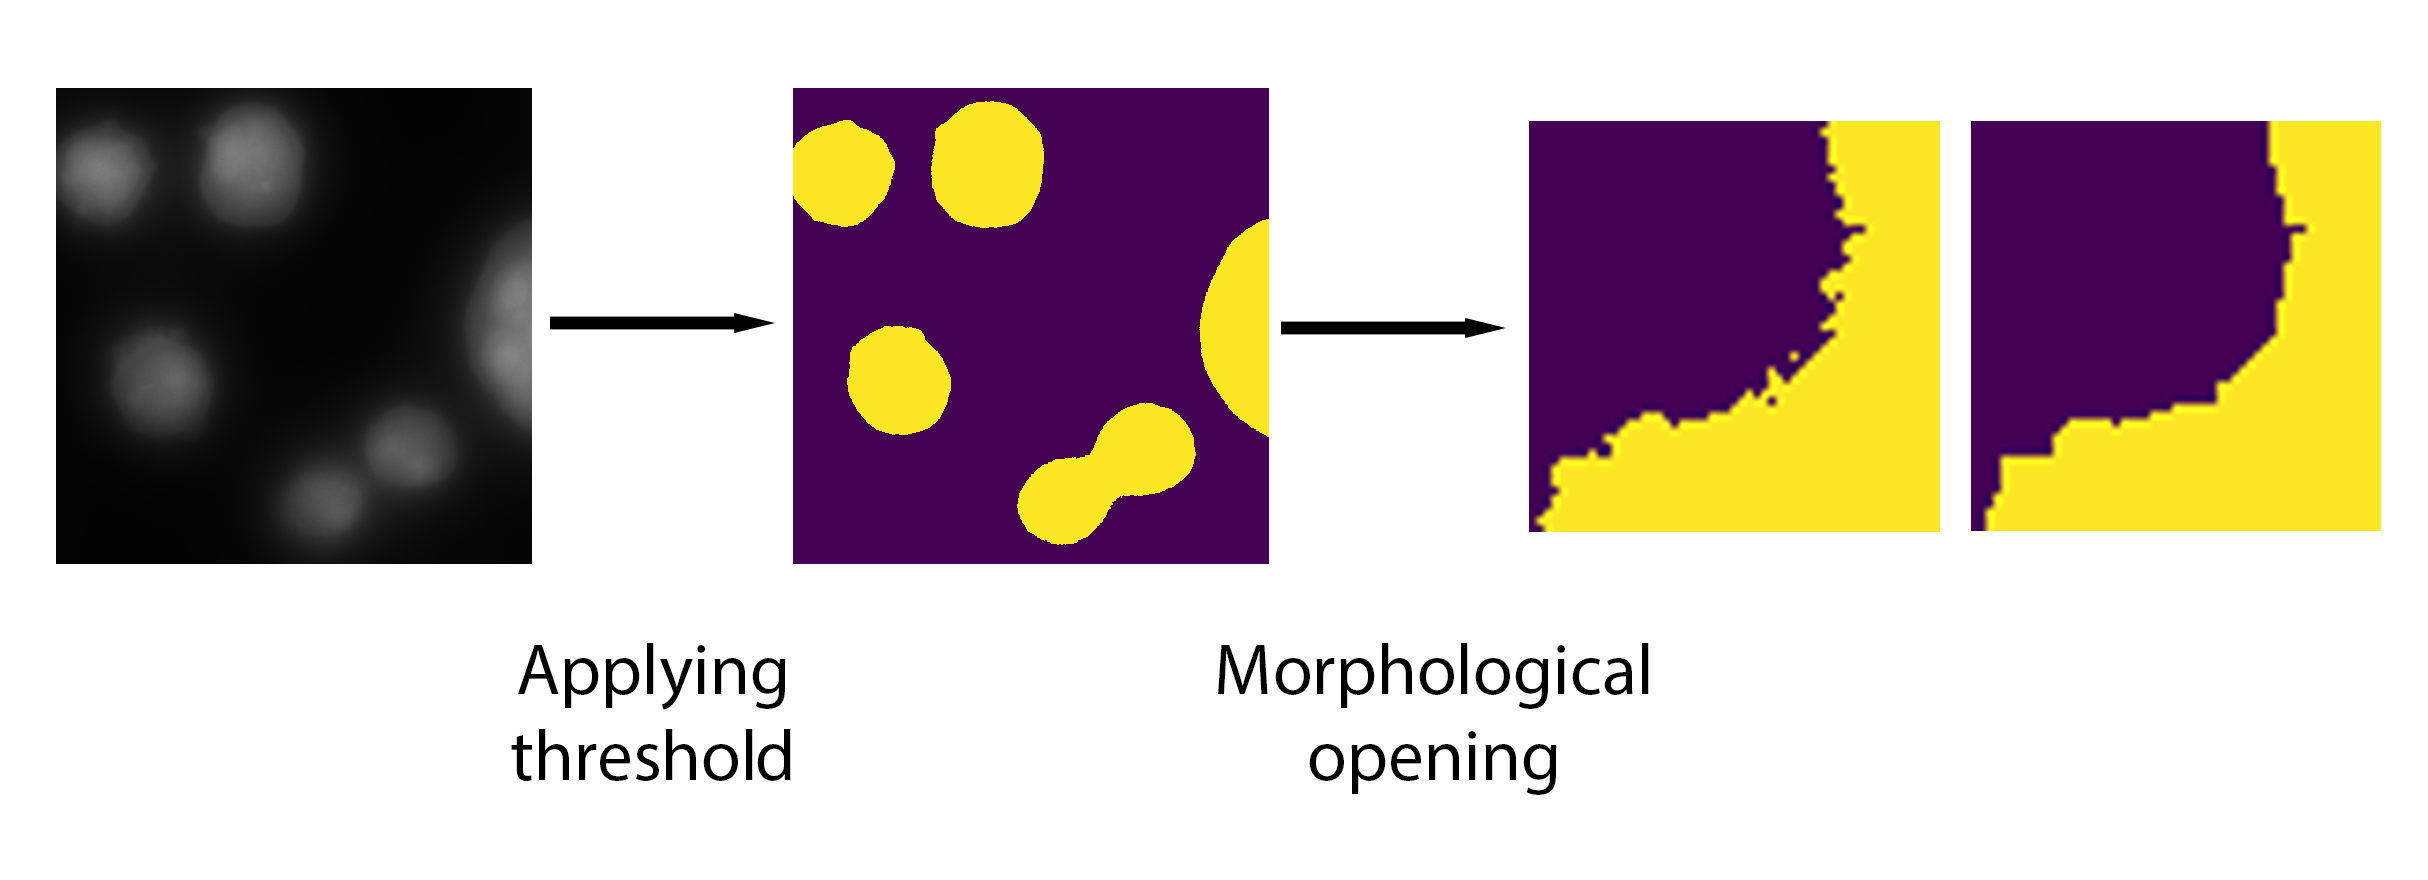
\includegraphics[width=0.5\linewidth]{bilder/gfp/binary-bce/preprocessing/preprocessing-gfp.png}
		\caption{Converting GFP into a binary mask}\label{fig:gfp-binary}
	\end{center}
\end{figure}

Figure \ref{fig:gfp-binary} displays the pipeline of converting an intensity image into a binary mask. After applying local threshold algorithm, additional morphological opening operation has been performed in order to smoothen the borders of the cell and remove noise. 